%%%%%%%%%%%%%%%%%%%%%%%%%%%%%%%%%%%%%%%%%%%%%%%%%%%%%%%%%%%%%%%%%%%%
%% I, the copyright holder of this work, release this work into the
%% public domain. This applies worldwide. In some countries this may
%% not be legally possible; if so: I grant anyone the right to use
%% this work for any purpose, without any conditions, unless such
%% conditions are required by law.
%%%%%%%%%%%%%%%%%%%%%%%%%%%%%%%%%%%%%%%%%%%%%%%%%%%%%%%%%%%%%%%%%%%%

\documentclass{beamer}
\usetheme[faculty=phil, logo = minerva.png]{fibeamer}
\usepackage[utf8]{inputenc}
\usepackage[
  main=english, %% By using `czech` or `slovak` as the main locale
                %% instead of `english`, you can typeset the
                %% presentation in either Czech or Slovak,
                %% respectively.
  czech, slovak %% The additional keys allow foreign texts to be
]{babel}        %% typeset as follows:
%%
%%   \begin{otherlanguage}{czech}   ... \end{otherlanguage}
%%   \begin{otherlanguage}{slovak}  ... \end{otherlanguage}
%%
%% These macros specify information about the presentation
\title{Um estudo sobre metódos simpléticos} %% that will be typeset on the
\subtitle{Solução Númerica do problema dos n-corpos} %% title page.
\author{Gil Sales M. Neto}
%% These additional packages are used within the document:
\usepackage{ragged2e}  % `\justifying` text
\usepackage{booktabs}  % Tables
\usepackage{tabularx}
\usepackage{tikz}      % Diagrams
\usetikzlibrary{calc, shapes, backgrounds}
\usepackage{amsmath, amssymb}
\usepackage{url}       % `\url`s
\usepackage{listings}  % Code listings
\frenchspacing
\begin{document}
  \frame{\maketitle}

  \AtBeginSection[]{% Print an outline at the beginning of sections
    \begin{frame}<beamer>
      \frametitle{Outline for Section \thesection}
      \tableofcontents[currentsection]
    \end{frame}}

    \section{Light Frames}
    \subsection{Blind Text}
    \begin{frame}{O Problema dos N-Corpos}
      \framesubtitle{}%
      O problema dos dois, três ou n-corpos é um problema de mecânica clássica ou mecânica quântica que modela o movimento de \(n\) partículas. O movimento é calculado utilizando as Leis de Movimento de Newton, e a Lei da Gravitação Universal de Newton.
    \end{frame}

    \begin{frame}{One Differential Equation to rule them all}
      \framesubtitle{One Differential Equation to FIND them all}%
      A segunda lei de Newton
      \[F = ma\]
      A Lei da Gravitação Universal
      \[F = G \cdot \frac{m_1 m_2}{r ^2}\]
      The One Differential equation
      \[
        \ddot{r} = G \cdot \frac{m_2}{\lVert r \rVert ^2}
      \]
    \end{frame}

    \begin{frame}{Redução de ordem da EDO e sistema de Equações}
      \framesubtitle{}%
      A equação diferencial
      \[
        \ddot{r_i} = G \cdot \sum_{j = 0}^{8}\frac{m_j}{\lVert r_{i,j} \rVert ^2}
      \]
      Reduzindo a um sistema de equações
      \[
      \begin{cases}
        \frac{\mathrm{d}r_i}{\mathrm{d}t} = v_i \\
        \frac{\mathrm{d}v_i}{\mathrm{d}t} = G \cdot \sum_{j = 0}^{8}\frac{m_j}{\lVert r_{i,j} \rVert ^2}
      \end{cases}
      \]
      E resolvendo esse sistema de equações podemos determinar a posição do corpo \(i\)
    \end{frame}

    \begin{frame}{As leis físicas que regem o movimento dos planetas}
      \framesubtitle{}%
      \begin{columns}[onlytextwidth]
        \column{.5\textwidth}
          As 3 leis de Kepler
          \begin{enumerate}
            \item Planetas se movem ao redor do Sol em órbitas Elipticas, com o Sol em um dos focos
            \item Um planeta varre a mesma área em um mesmo período de tempo
            \item Os quadrados dos períodos de revolução dos planetas são diretamente proporcionais aos cubos dos raios médios de suas órbitas
          \end{enumerate}
        \column{.4\textwidth}
        Conservação de Energia Mecânica e Momento Angular
        \begin{itemize}
          \item \(E = K_e + P_e\)
          \item \(\frac{\mathrm{d}E}{\mathrm{d}t} = 0 \)
          \item \(L = r \times p\)
          \item \(\frac{\mathrm{d}L}{\mathrm{d}t} = 0 \)
        \end{itemize}
      \end{columns}
    \end{frame}

    \begin{frame}{Discretização da EDO}
      \framesubtitle{O Metódo de Euler}%
      Podemos discretizar a nossa equação diferencial com base no metódo de Euler, que é um metódo de passo explicito.\\
      A discretização é feita com a expansão em Série de Taylor das equações diferenciais
      \[
      \begin{cases}
        r_{t+1} = r_{t} + \Delta t \cdot v_t\\
        v_{t+1} = v_{t} + \Delta t \cdot a_t
      \end{cases}
      \]
    \end{frame}

    \begin{frame}{Visualizando a solução}
      \framesubtitle{A órbita dos planetas}%
      \begin{figure}[h]
        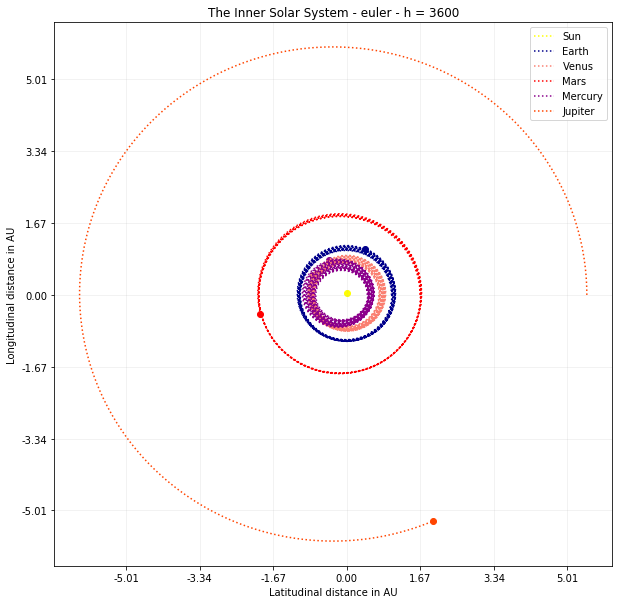
\includegraphics[width=90mm, height = 70mm]{resources/euler-3600-orbit.png}
      \end{figure}
    \end{frame}

    \begin{frame}{O que deu errado?}
      \framesubtitle{Integradores Simpléticos}%
      O metódo de Euler explicito conserva apenas aproximadamente a energia do sistema.\\
      Metódos simpléticos conservam exatamente uma quantia que aproximadamente é a Energia.\\
      \caption{Leapfrog Integrators}
      \begin{itemize}
        \item Euler-Cromer
        \item 3 Step Verlet
        \item 7 Step Verlet
      \end{itemize}
    \end{frame}

    \begin{frame}{Euler-Cromer}
      \framesubtitle{Verlet-Stormer}%
      \[
      \begin{cases}
        v_{t+1} = v_{t} + \Delta t \cdot a_t\\
        r_{t+1} = r_{t} + \Delta t \cdot v_{t+1}
      \end{cases}
      \]
    \end{frame}

    \begin{frame}{Integrador de Verlet de 3 passos}
      \framesubtitle{Velocity Verlet}%
      \[
      \begin{cases}
        v_{t_\frac{1}{2}} = v_t + \frac{1}{2} \Delta t \cdot a_t  \\
        r_{t+1} = r_t + \Delta t \cdot v_{t\frac{1}{2}} \\
        v_{t+1} = v_{t\frac{1}{2}} + \frac{1}{2}\Delta t\cdot A(r_{t+1})
      \end{cases}
      \]
    \end{frame}

    \begin{frame}{Integrador de Verlet de 7 passos}
      \framesubtitle{Leapfrog}%
      \begin{columns}[onlytextwidth]
        \column{.5\textwidth}
      \[
      \begin{cases}
        w &= \sqrt[3]{2}\\
        f &= 2 - w\\
        leap_1 = leap_7 &= \frac{h}{2f}\\
        leap_2 = leap_6 &= \frac{h}{f}\\
        leap_3 = leap_5 &= (1-w) \frac{h}{2f}\\
        leap_4 &= -h \frac{w}{f}
      \end{cases}
      \]
      \column{.5\textwidth}
      \[
      \begin{cases}
      x_{1} &= x_t + leap_1 \cdot v_t\\
      v_{2} &= v_t + leap_2 \cdot A(x_{1})\\
      x_{3} &= x_{1} + leap_3 \cdot v_{2}\\
      v_{4} &= v_{2} + leap_4 \cdot A(x_{3})\\
      x_{5} &= x_{3} + leap_5 \cdot v_{4}\\
      v_{t+1} &= v_{4} + leap_6 \cdot A(x_{5})\\
      x_{t+1} &= x_{5} + leap_7 \cdot v_{t+1}
    \end{cases}
    \]
    \end{columns}
    \end{frame}

    \begin{frame}{Muito Obrigado!}
      \framesubtitle{Inspirado no texto de Carl Sagan}

      \begin{block}{}
        Diante da vastidão do \alert{tempo} e da imensidão do \alert{universo}, é um prazer para mim dividir um \alert{planeta}, uma \alert{época} e uma \alert{matéria} com vocês.
      \end{block}
    \end{frame}
\end{document}
